
\section{Perceiving the body in action}

Motion of the arm may generate optic flow directly through the
changing projection of the arm itself, or indirectly through an object
that the arm is in contact with.  While the relationship between the
optic flow and the physical motion is likely to be complex,
the correlation in time of the two events should be
exceedingly precise.  This time-correlation can be used as a
``signature'' to identify parts of the scene that are being influenced
by the robot's motion, even in the presence of other distracting
motion sources.  In this section, we show how this tight correlation
can be used to localize the arm in the image without any prior
information about visual appearance.  
%%In the next section we will show
%%that once the arm has been localized we can go further, and identify
%%the boundaries of objects with which the arm comes into contact.

\subsubsection*{Reaching out}

The first step towards manipulation is to reach objects within the
workspace.  If we assume targets are chosen visually, then ideally we
need to also locate the end-effector visually to generate an error
signal for closed-loop control.  Some element of open-loop control is
necessary since the end-point may not always be in the field of view
(for example, when it is in its resting position), and the overall
reaching operation can be made faster with a feed-forward contribution
to the control.

\begin{figure}[tb]
\begin{center}
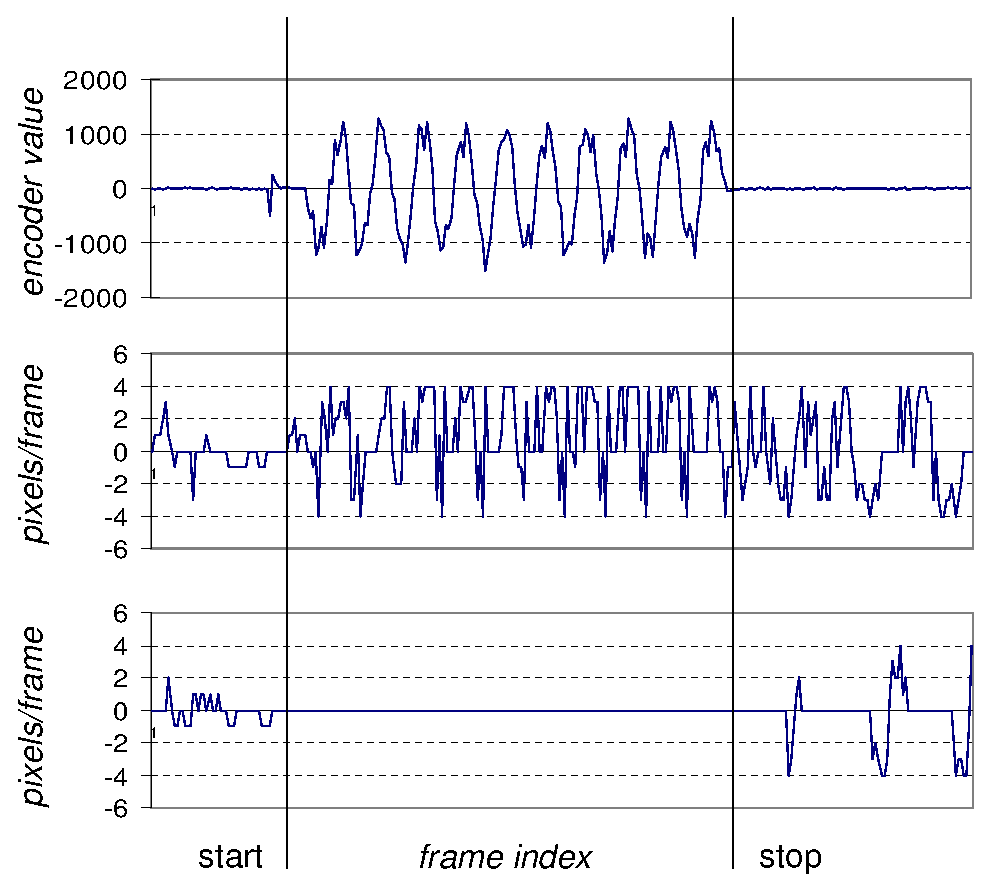
\includegraphics[width=6.0cm]{joint-correlation3.eps}
%%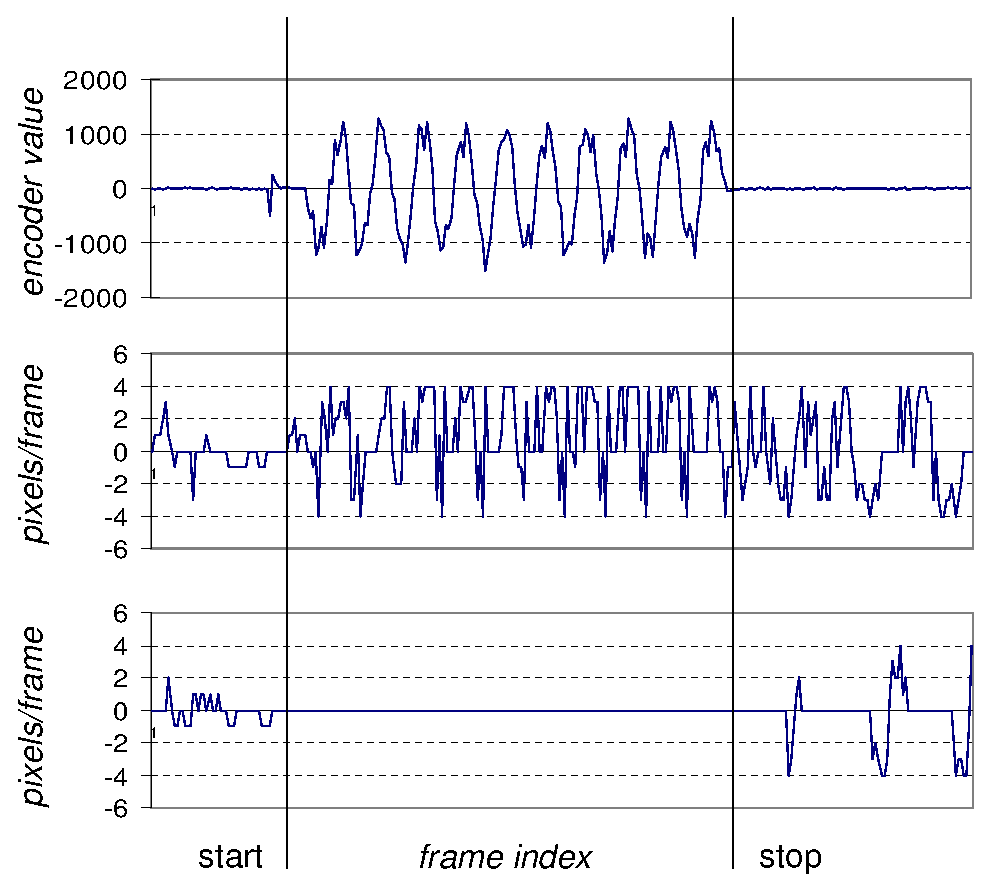
\includegraphics[width=\columnwidth]{joint-correlation3.eps}
\caption{ 
\label{fig:joint-correlation}
%
An example of the correlation between optic flow and arm movement.
The traces show the movement of the wrist joint (upper plot)
and optic flow sampled on the arm (middle plot) and away from it (lower
plot).  As the arm generates a repetitive movement, the oscillation
is clearly visible in the middle plot and absent in the lower.
Before and after the movement the head is free to saccade, generating the
other spikes seen in the optic flow.
%
}
\end{center}
\end{figure}


The simplest possible open loop control would map directly from a
fixation point to the arm motor commands needed to reach that point
\cite{metta99developmental} using a stereotyped trajectory, perhaps
using postural primitives \cite{mussa-ivaldi92vector}.  If we can
fixate the end-effector, then it is possible to learn this map by
exploring different combinations of direction of gaze vs.  arm
position \cite{Marjanovic-96-SAB,metta99developmental}.  So locating
the end-effector visually is key both to closed-loop control, and to
training up a feed-forward path.  We shall demonstrate that this
localization can be performed without knowledge of the arm's appearance,
and without assuming that the arm is the only moving object in the
scene.

\ifverbose
NEW The closed loop control requires the identification of both the
end-effector and the target in the image plane. As in the visual
servoing literature \cite{espiau92new} it is certainly possible to
design a feedback controller based on the knowledge of the Jacobian
mapping between the image and the robot joint space -- globally
represented by both the position of the cameras in space and the arm.
The state space in our case is 13-dimensional. Constructing the
Jacobian requires the calibration of the robot and the estimation of
the kinematics.  On the other hand, for the configurations where the
object and the end-point are close one to the other, it is possible to
simplify the formulation by assuming the controller is locally
constant with respect to the arm position (this removes 6 dimensions).
Still the controller is a function of the configuration of the head.
This dependency must be roughly taken into account to move the arm
correctly. The requirements in terms of precision are in fact not that
stringent because what matters for the closed loop controller is that
the sign remains negative with respect to the visual error. For our
purpose this relationship can be learned by the same exploration
procedure mentioned above for the open loop controller.  For both
controllers the problem translates into localizing the arm's end-point
in the image plane. We shall demonstrate that visual localization can
be performed without relying on a particular \ahhcolor{} or pattern but
simply on movement and motor information.
\fi

\begin{figure}[tb]
\begin{center}
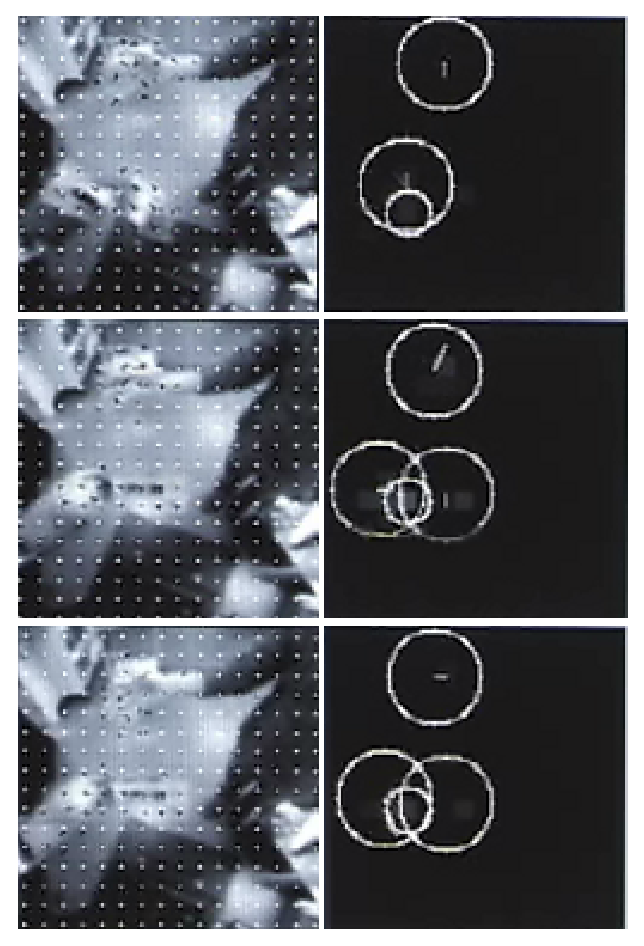
\includegraphics[width=5cm]{arm-detection2.eps}
\caption{ 
\label{fig:arm-detection}
%
Detecting the arm/gripper through motion correlation. The robot's
point of view and the optic flow generated are shown on the left. On
the right are the results of correlation.  Large circles represent the
results of applying a region growing procedure to the optic flow.
Here the flow corresponds to the robot's arm and the experimenter's
hand in the background. The small circle marks the point of maximum 
correlation, identifying the regions that correspond to the robot's own arm.
%
}
\end{center}
\end{figure}


\subsubsection*{Localizing the arm visually}

The robot is not a passive observer of its arm, but rather the
initiator of its movement.  This can be used to distinguish the arm
from parts of the environment that are more weakly affected by the
robot.  The arm of a robot was detected in \cite{Marjanovic-96-SAB} by
simply waving it and assuming it was the only moving object in the
scene.  We take a similar approach here, but use a more
stringent test of looking for optic flow that is correlated with
the motor commands to the arm.  This allows unrelated movement
to be ignored.  Even if a capricious engineer were to 
replace the robot's arm with one of a very different appearance,
and then stand around waving the old arm, this detection method
will not be fooled.  

The actual relationship between arm movements and the optic flow they
generate is complex.  Since the robot is in control of the arm, it can
choose to move it in a way that bypasses this complexity.  In
particular, if the arm rapidly reverses direction, the optic flow at
that instant will change in sign, giving a tight, clean temporal
correlation.  Since our optic flow processing is coarse (a $16\times
16$ grid over a $128\times 128$ image at 15 Hz), we simply repeat this
reversal a number of times to get a strong correlation signal during
training.  With each reversal the probability of correlating with
unrelated motion in the environment goes down.  
%%This probability could
%%also be reduced by higher resolution (particularly in time) visual
%%processing.

\ifverbose
Localizing the robot arm is not the same as searching into the visual
space for a generic object we do not have any expectancy on its
whereabouts. The robot can exploit the fact it looks for its own body
part to self-generate useful cues to help the localization. The
fundamental idea is to cross-correlate the presence of motion in the
image with the actual arm motion as sensed through proprioception (or
efference copy). When the two quantities have a positive correlation
over a given time window, we can assert that that image location
belongs to the visual projection of the arm. From the visual point of
view, the optic flow can be used. We employed a block matching
technique over a 16x16 grid out of a 128x128 pixels image.
\fi


\ifverbose
\begin{figure}[tb]
\begin{center}
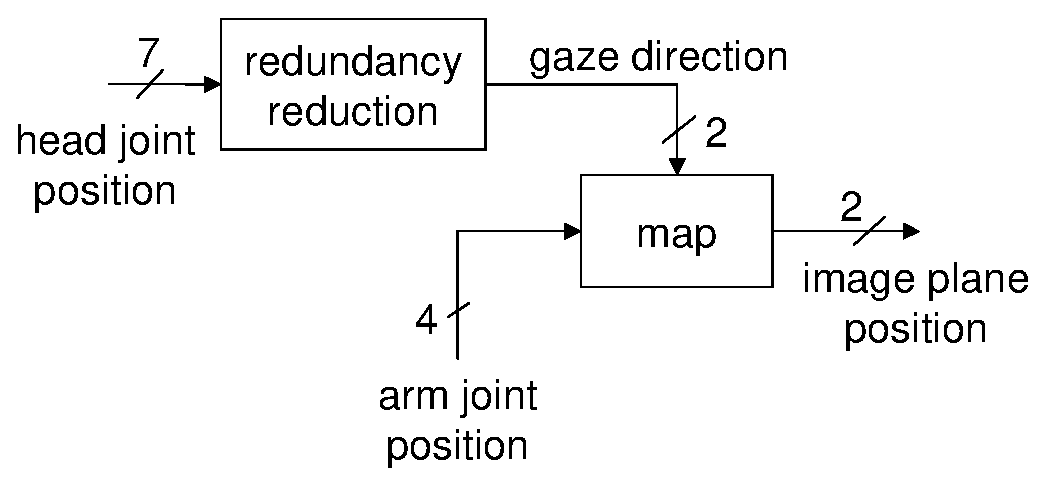
\includegraphics[width=\columnwidth]{mapping-reach.eps}
\caption{ 
\label{fig:mapping-reach}
%
Mapping from proprioceptive input to a visual prediction. Head and arm
joint positions are used to estimate the position of the projection of
the hand in the image plane.  Redundant configurations of the (7 DOF)
head are mapped to a simpler (2D) representation, and the wrist-related 
DOFs of the arm are ignored.
%
}
\end{center}
\end{figure}
\fi

\ifverbose
These two ideas were exploited contextually. The cross-correlation
runs on a 500ms time window while the robot generates a relatively
high-frequency movement. The resulting correlation array (each pixel
is correlated with all joints) is post-processed by a thresholding
procedure and subsequently by a region-growing algorithm. Regions are
identified and labeled. The arm position is identified as the center
of mass of the region containing the maximum of the correlation
function.
\fi

Figure~\ref{fig:joint-correlation} shows an example of this procedure
in operation, comparing the velocity of the arm's wrist with the optic
flow at two positions in the image plane.  A trace taken from a
position away from the arm shows no correlation, while conversely the
flow at a position on the wrist is strongly different from zero over
the same period of time.  Figure~\ref{fig:arm-detection} shows
examples of detection of the arm and rejection of a distractor.


\subsubsection*{Localizing the arm using proprioception}

The localization method for the arm described so far relies on a
relatively long ``signature'' movement that would slow down reaching.
This can be overcome by training up a function to estimate the
location of the arm in the image plane from proprioceptive information
(joint angles) during an exploratory phase, and using that to 
constrain arm localization during actual operation.
%%As a function approximator we simply fill a look-up table,
%%reducing the 11-dimensional input space of joint angles based on 
%%the much lower number of degrees of freedom used in controlling them
%%(see Figure~\ref{fig:mapping-reach}).
Figure~\ref{fig:predict-position} shows the resulting \ahhbehavior{}
after about twenty minutes of real-time learning. 
%
\ifverbose
Note as both the
position of the arm and the direction of gaze change in these
examples: the position of objects such as the base of the robot at the
bottom of the image varies.
\fi
%
\ifverbose
We can imagine building a function from examples to predict the
position of the arm/end-point in the image plane. Examples are
collected when the arm is localized and have the form of joint
space-image coordinates [equation here?]. In principle a very big
lookup table can be used. The problem is that the input space is
13-dimensional (7 degrees of freedom describing the head configuration
and 6 describing the arm position), and nearest neighbor lookup tables
are known to work poorly in highly dimensional spaces. Beside,
collecting enough samples to span the space densely enough might
require a very long time. We can observe though that only the first
four arm joints determine the appearance of the end-point in the image
plane (the wrist is irrelevant), and the position in space of the
image plane although determined by the head configuration can be
described by only two numbers. These two parameters describe only the
orientation and not the position in space. In theory a distance factor
should be also considered, but it would only marginally influence the
map because the change in distance of the arm with respect to the
camera is small for the allowed movement of the head/arm [hope I
convinced the audience].
\fi


\ifverbose
Can we determine which is the set of redundant configuration of the
head for each given orientation of the camera? We can indeed spot when
two orientations of the camera are the same in spite of the head
configuration been different: this is true if the following statements
are true:
%
\begin{itemize}
%
\item Projection of the arm end-point in the image plane.
%
\item Arm joint position.
%
\item The head configurations are different.
%
\end{itemize}
%
Whenever a new data point (input/output) is used for training, it is
checked against all existing elements in the lookup table. If any of
them satisfy the above-mentioned conditions it is not inserted as a
new point but rather as belonging to the same camera direction.
Figure~\ref{fig:mapping-reach} depicts a schematic of the map as
implemented.

\fi

\ifverbose
\section{Putting things together}

Figure 6 shows how all components of the reaching subsystem are put
together. The lowest level controller is a double loop consisting of a
torque loop based on the reading of the joint strain gauges, and a
position/velocity feedback loop based on the potentiometer readings.
Depending on the tuning of the position/velocity gain it is possible
to obtain a low stiffness yet precise enough controller. Our tuning in
fact has a low positional gain and a relatively higher velocity gain.
The \ahhbehavior{} is thus that of a low-stiffness controller with still a
good \ahhbehavior{} when closing a velocity loop [unclear].

The successive level above is a simple linear combination of postural
primitives. There are four primitives in the present implementation,
which span a good portion of the arm workspace frontal to the robot
chest. Primitives are defined in joint space.

Oscillatory movements are generated by a specific subsystem in
parallel to the postural primitives block. Oscillations are created by
specifying directly the speed of the arm joints.

Further up in the control chain there is the open loop controller.
This is implemented as a nearest neighbor lookup table mapping the
gaze direction into a set of coefficient. The coefficients are the
weights of the linear combination of postural primitives.

The arm locator algorithms control in different ways both the
generation of appropriate movements for the self-localization and the
switching between different control regimes (not indicated in figure).

There are two caveats: first, an additional and more precise visual
bit of information is probably needed, and second, the closed loop
controller has not been implemented yet. The former issue can probably
be solved by looking for a gray blob close to the predicted arm
position. Once the position of the end-point is accurately estimated,
a reliable closed loop controller can be learned and employed after the
open loop to bring the flipper in contact with the target object.
\fi

\ifverbose
\begin{figure}[tbh]
\begin{center}
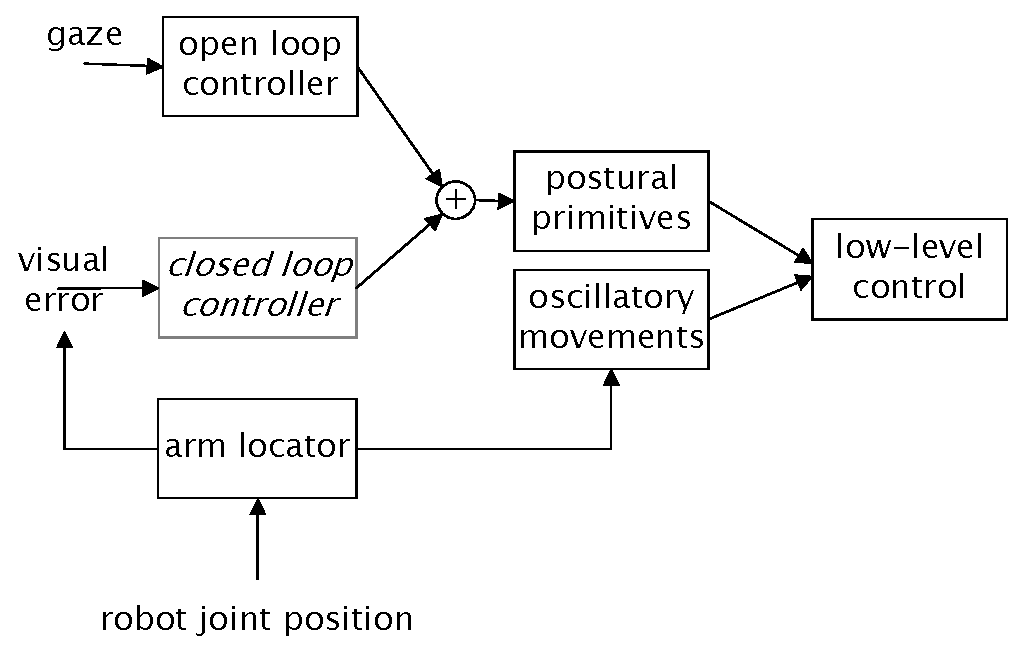
\includegraphics[width=\columnwidth]{control-flow.eps}
\caption{ 
\label{fig:control-flow}
%
  The controller.  Probably have to bring back text to describe this
  if we include this figure.
%
}
\end{center}
\end{figure}
\fi

\begin{figure}[tb]
\begin{center}
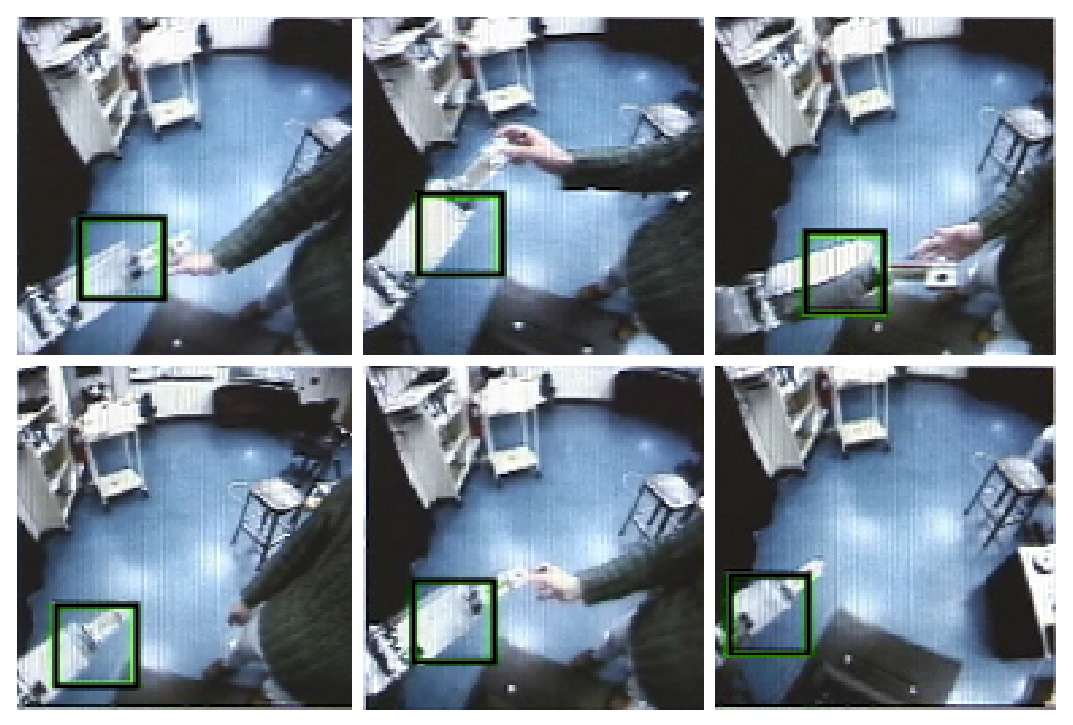
\includegraphics[width=6.0cm]{predict-position.eps}
%%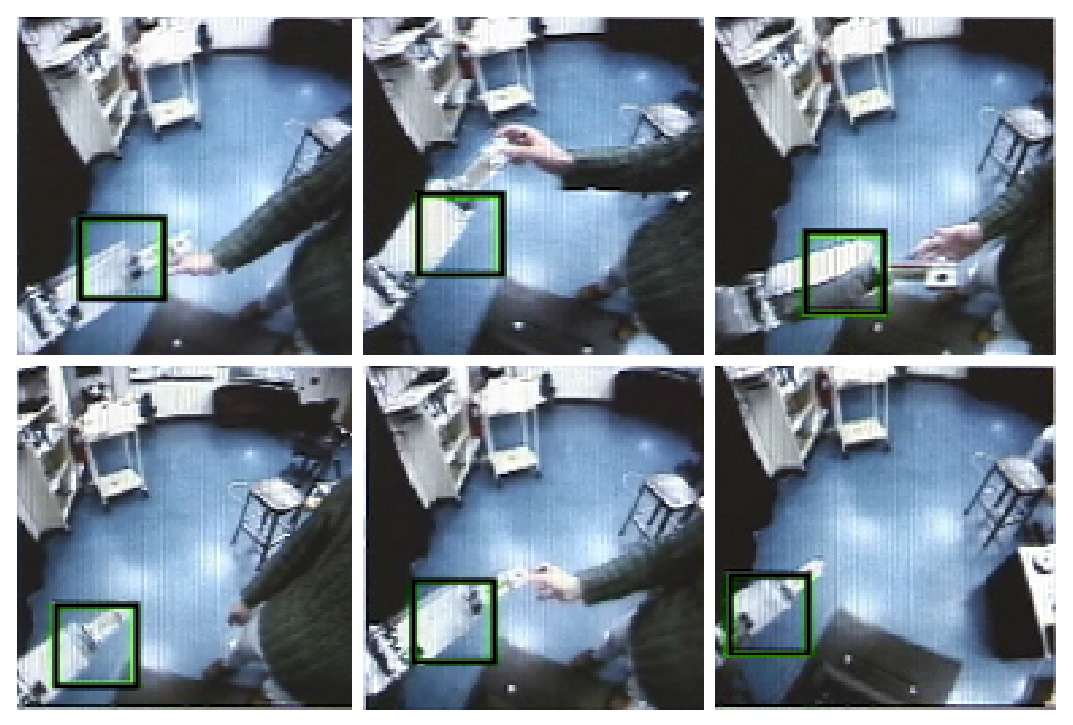
\includegraphics[width=\columnwidth]{predict-position.eps}
\caption{ 
\label{fig:predict-position}
%
Predicting the location of the arm in the image as the head and arm
change position. The rectangle represents the predicted position of
the arm using the map learned during a twenty-minute training run.
The predicted position just needs to be sufficiently accurate to
initialize a visual search for the exact position of the end-effector.
%
}
\end{center}
\end{figure}

